\begin{figure}
  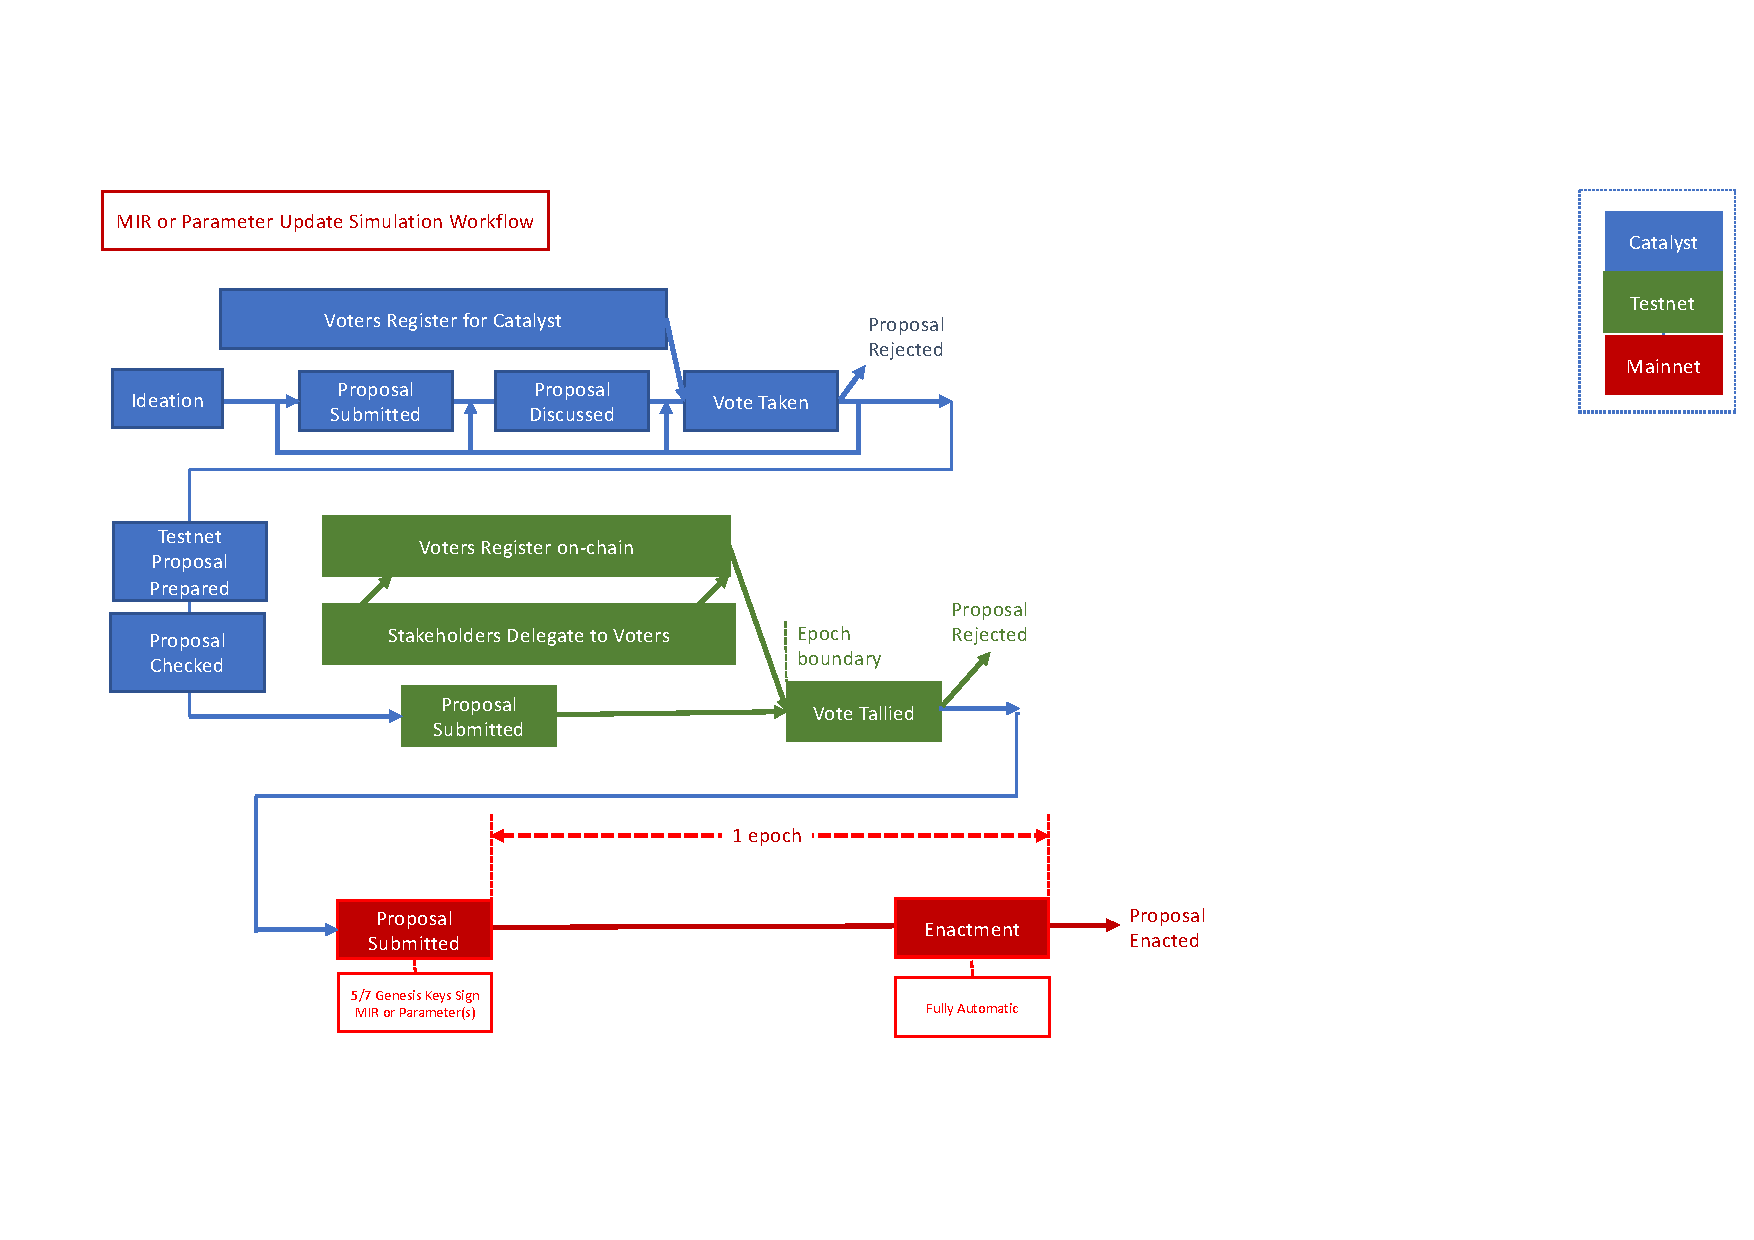
\includegraphics[trim=0 90 0 80,clip,width=\textwidth]{Workflow1}
  \caption{Example Workflow: Funds Transfer (MIR) or Simple Parameter Value Update}
  \label{fig:workflow-mir}
\end{figure}

\section{Example Workflows}
\label{sec:workflows}

Figures~\ref{fig:workflow-mir}-\ref{fig:workflow-hf} show outline workflows for
typical use cases.  Figure~\ref{fig:workflow-mir} shows the workflow that is
involved in submitting either a proposal to transfer funds, or to change the
value of an updatable protocol parameter.  Figure \ref{fig:workflow-hf} shows
the corresponding workflow for a protocol version change (``hard fork'').

\paragraph{Parameter Updates and Funds Transfers.}  Parameter update and funds transfer proposals involve three main stages:
proposal submission, on-chain voting, and proposal enactment.  In the workflow that is described
here, proposal preparation, proposal submission, delegate registration,
vote delegation and voting involve manual steps, but stake snapshots, vote tallying
and enactment are fully automatic.  Stake snapshots are taken at each epoch boundary.
These govern the weight of each vote delegation during the upcoming epoch.
%
Delegates may register at any time.  Ada holders may delegate to any registered delegate.
Delegates may choose to vote on any active proposal prior to the specified vote deadline.
Following the deadline, all votes are tallied.  If a proposal does not receive sufficient vote, then
it will be automatically rejected.  Otherwise, it is automatically accepted, and passed on for
automatic enactment.
In order to ensure the stability of the chain, voting must be completed sufficiently before the update takes
effect.  This period has been fixed at \texttt{LatestVotingDeadline} slots prior to the epoch where the proposed is enacted.\todo{Determine this setting!}

\begin{figure}
  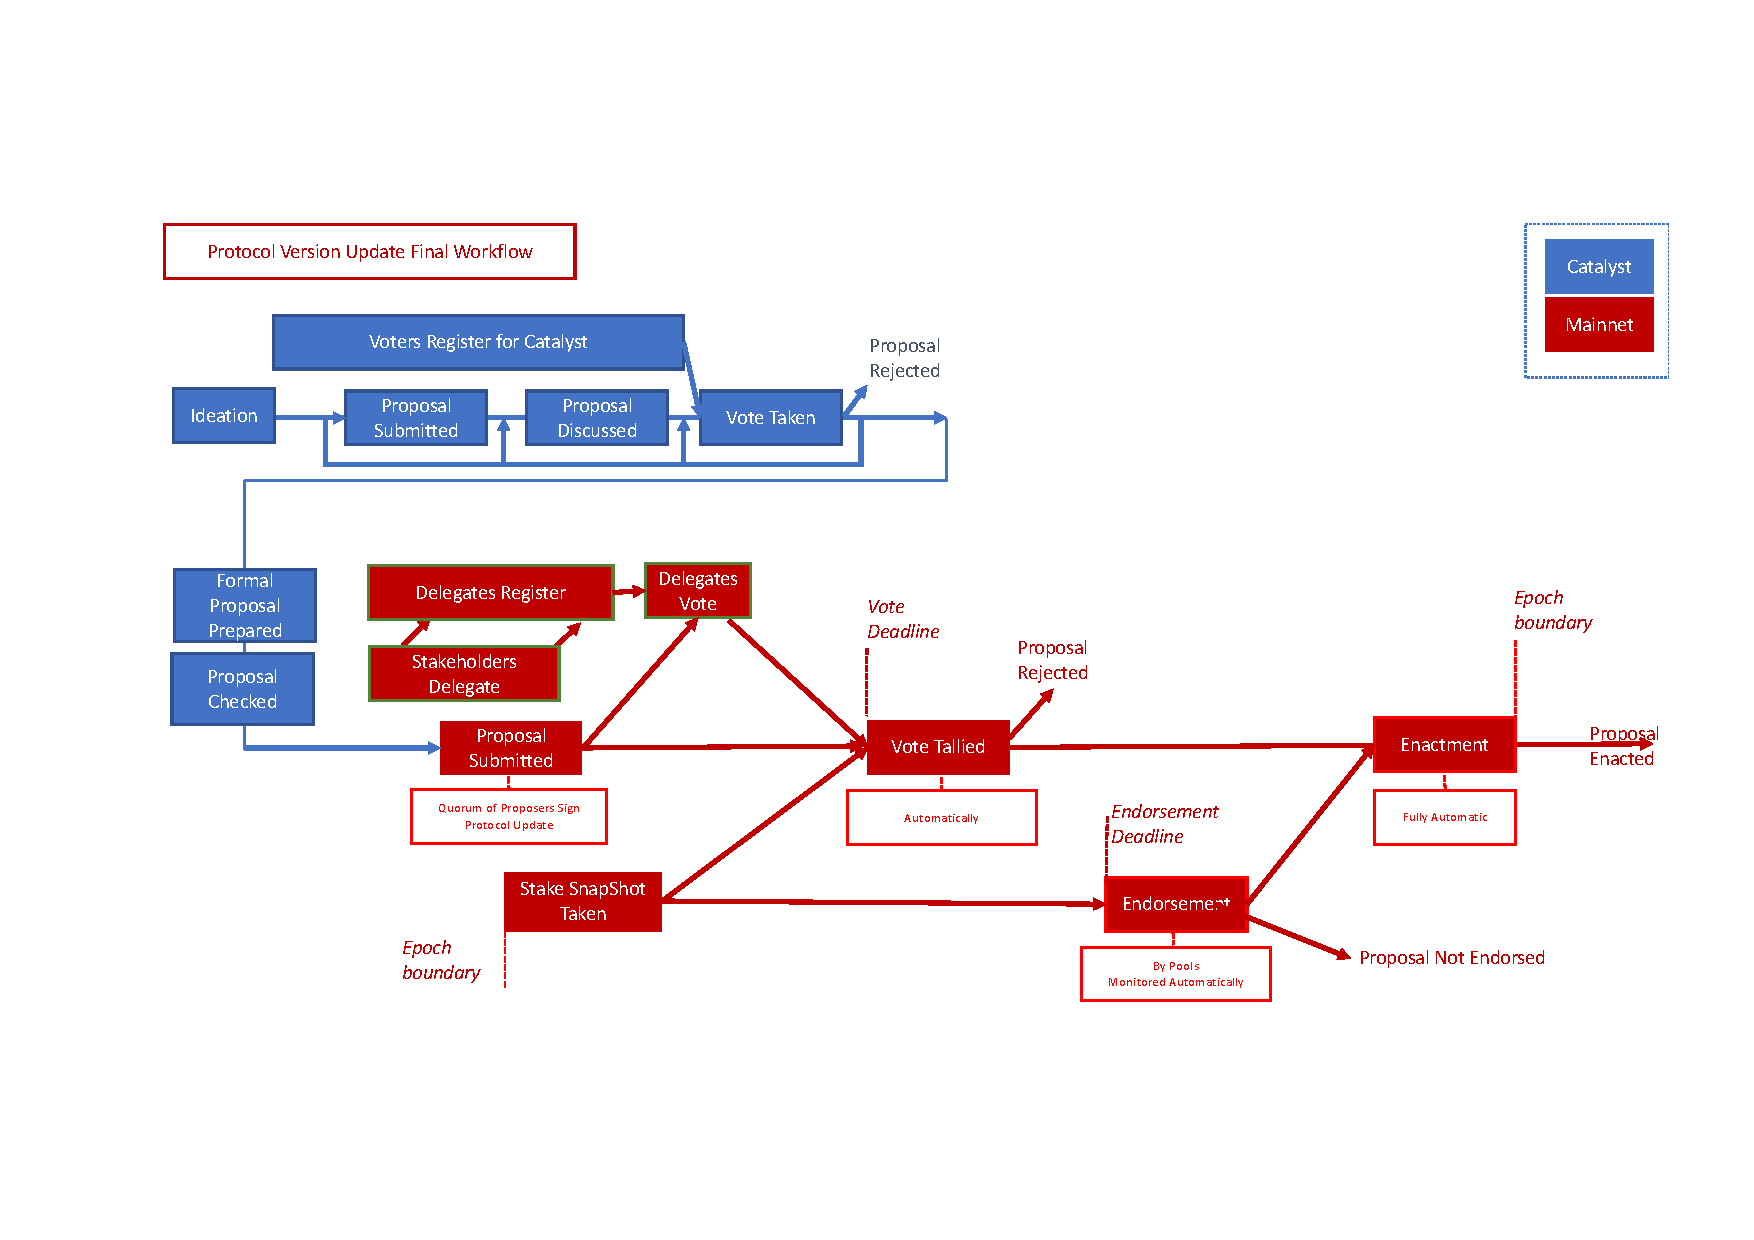
\includegraphics[trim=0 90 0 80,clip,width=\textwidth]{New-Workflow2}
  \caption{Example Workflow: Protocol Version Update (Hard Fork)}
  \label{fig:workflow-hf}
\end{figure}

\paragraph{Protocol Version Updates (Hard Forks).}  These follow the process described above,
except that the proposal must also be \emph{endorsed} by sufficient block-producing stake
(where endorsement indicates the readiness of the stake pool operator to upgrade to the new protocol version).
The same process applies to both major and minor protocol version upgrades.
The deadline for endorsement must be given in the original proposal submission.
In order to ensure the stability of the chain, endorsement must happen sufficiently before the update takes
effect.  This has been fixed at \texttt{LatestEndorsementDeadline} slots prior to the epoch where the proposed is enacted.\todo{Determine this setting!}
If a proposal does not pass the endorsement threshold then it will be rejected at this point, otherwise it will be
passed on for automatic enactment.  It is anticipated that endorsement will be automatic, based on the percentage of stake that
is controlled by upgraded stake pools.
% through manual confirmation by each stake pool operator, though it would be possible
% to automate this by monitoring software versions.\khcomment{Jared has defined an automated process.}
While the endorsement deadline will usually be after the voting deadline, this is not technically necessary, and the deadlines could
in principle be contemporaneous, or even reversed.

\paragraph{Rejected Proposals.}   Once it has been rejected, a proposal is never enacted on-chain.
An equivalent proposal may, however, be submitted, in which case the new proposal must go through the same voting and enactment process
as the original proposal (and may, itself, be rejected).
